%% Beispiel-Präsentation mit LaTeX Beamer im KIT-Design
%% entsprechend den Gestaltungsrichtlinien vom 1. August 2020
%%
%% Siehe https://sdqweb.ipd.kit.edu/wiki/Dokumentvorlagen

%% Beispiel-Präsentation
\documentclass[en]{sdqbeamer} 
\usepackage{graphicx}
\usepackage{hyperref}
\usepackage{subcaption}
\usepackage{multirow}
\hypersetup{
    colorlinks=true,
    linkcolor=gray,
    filecolor=magenta,      
    urlcolor=black,
    pdftitle={Overleaf Example},
    pdfpagemode=FullScreen,
    }

\urlstyle{same}
 
%% Titelbild
\titleimage{banner_2020_kit}

%% Gruppenlogo
\grouplogo{KIT_STAT_Logo_rgb.png} 

%% Gruppenname und Breite (Standard: 50 mm)
\groupname{}
%\groupnamewidth{50mm}

% Beginn der Präsentation

\title[Simple Prediction Intervals]{Simple Macroeconomic Forecast Distributions}
\subtitle{} 
\author[Friederike Becker, Fabian Krüger, Melanie Schienle]{Friederike Becker, Fabian Krüger, Melanie Schienle}

\date[30.\,07.\,2024]{July 30, 2024}


% Literatur 
 
\usepackage[citestyle=authoryear,bibstyle=numeric,hyperref,backend=biber]{biblatex}
\addbibresource{presentation.bib}
\bibhang1em

\begin{document}
\setbeamertemplate{caption}{\raggedright\insertcaption\par}
 
%Titelseite
\KITtitleframe

%Inhaltsverzeichnis
\begin{frame}{Overview}
\tableofcontents
\end{frame}

\section{Setting}


%\subsection{Fixed-Event forecasting in Economics}
\begin{frame}{An economist's favorite pastime}
	\begin{itemize}
	    \item various institutions issue forecasts for annual macroeconomic targets
     \begin{itemize}
        \item most prominent targets: (real) GDP growth and inflation
        \item for Germany, sources are (among others) the Bundesbank, the ifo institute, the OECD
         \item fixed-event forecasts: target date is fixed, forecast date is not
     \end{itemize}
     \item forecasts are often disseminated widely
     \begin{itemize}
         \item extensive media coverage, influence on political discussions
         \item relevant for real-world outcomes (public budget planning, collective bargaining)
     \end{itemize}
	\end{itemize}
\end{frame}

\begin{frame}[t]{Can we really be that sure?}

\begin{columns}
\begin{column}{0.4\textwidth}
   	\begin{itemize}
         \item usual practice: issue point forecasts only
         \begin{itemize}
	    \item uncertainty is at best acknowledged, rarely quantified \bigskip
	\end{itemize}
        %\item media reception often fixated on zero
        \item forecasts of different horizons are often left uncontextualized \bigskip
        \item distributional forecasts supposedly would require extra modeling effort
    \end{itemize}
    \vspace{2cm}
\end{column}
\begin{column}{0.6\textwidth}
    \begin{figure}
        \centering
        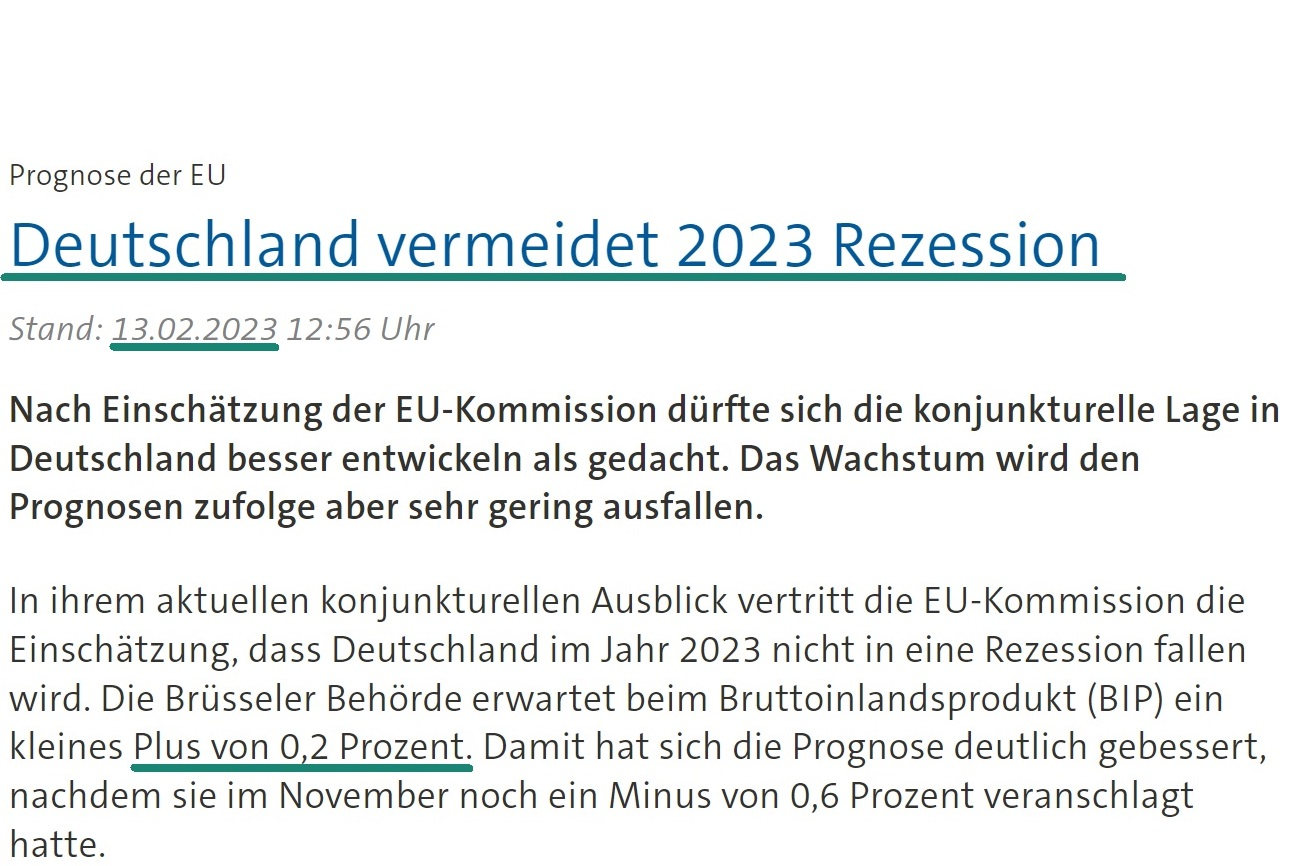
\includegraphics[width=0.8\textwidth]{figures/recession_light_underlined_green_smaller_date.jpg} 
        \caption{Source: tagesschau.de}
        \label{fig:enter-label}
    \end{figure}     
\end{column}
\end{columns}
\end{frame}

\begin{frame}[t]{Contributions of this work}
\begin{itemize}
    \item show that attaching prediction intervals to an existing base of point forecasts can be 
    \begin{itemize} 
    \item simple
    \item cheap
    \item transparent
    \end{itemize}   
    \item provide competitively performing distributional forecasts for 
    \begin{itemize}
    \item  GDP growth and inflation
    \item  all G7 countries
    \item  current and next year targets
    \end{itemize}
    %\item simple and transparent method of attaching prediction intervals 
%\item show that attaching distributional forecasts to an existing
%\item for up to one and a half years into the future 
%\item evaluate on years 1999-2021
\end{itemize}
\end{frame}

% \begin{flushright}
% 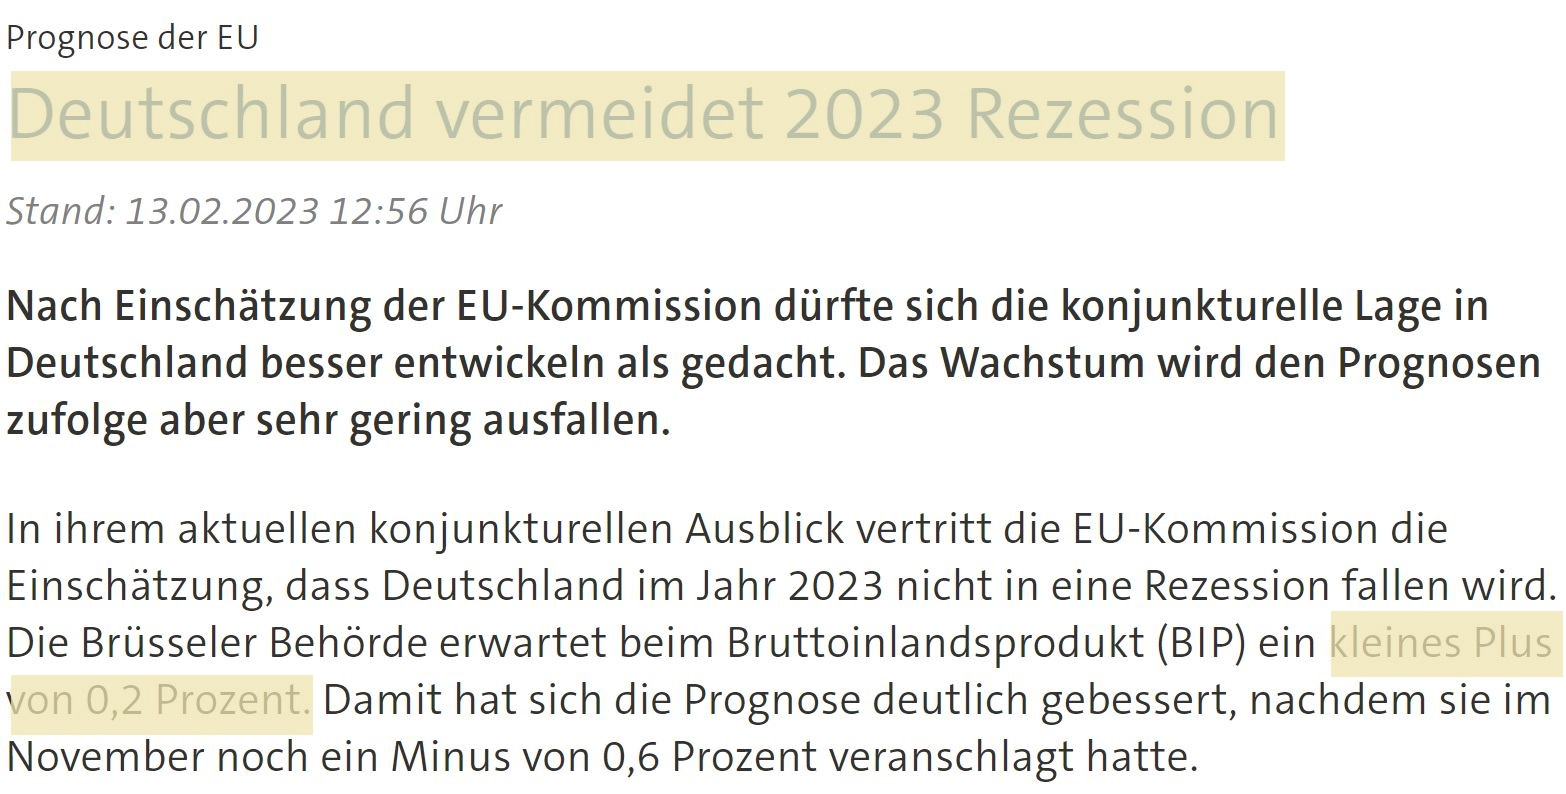
\includegraphics[width = 8cm]{figures/recession_light.JPG}    
% \end{flushright}
   
%\subsection{Data Source: IMF World Economic Outlook}
\begin{frame}{Data Source: IMF World Economic Outlook}
	\begin{itemize}
		\item survey by the IMF staff, published bi-annually
		\begin{itemize}
            \item contains forecasts with up to 6 years horizon and historic truth values
		    \item publication in April (horizon for current year $\approx$ 8 months) and in October ($\approx$ 2 months)
		\end{itemize}
    \item publicly available\footnote{International Monetary Fund. 2024. \textit{World Economic Outlook Database}, available at \url{https://www.imf.org/en/Publications/WEO/weo-database/2024/April}} in an accessible format
    \item targets: real GDP growth, CPI inflation, current account balance
    \item time range: available since 1990, giving $>$30 years of forecast-truth pairs %per country and forecast horizon
    \item target locations: forecasts are issued for 196 countries in total
    %\begin{itemize}
    %    \item forecasts for 196 countries in total are available
    %\end{itemize}
	\end{itemize}
\end{frame}

\section{Methods}
\begin{frame}{Methods}
We apply an attractively simple and cheap method. For a given country and target:
\begin{itemize}
    \item given forecasts $\hat{y}_{t, h}$ and the realized true values $y_{t}$ ...
    \begin{itemize}
        \item for target year $t$, horizon $h$
    \end{itemize}
    \item ... construct sets $\mathcal{E}_{t, h} = \{\hat{e}^{abs}_{t^*, h}  | t-R \leq t^* < t \}$, containing the last $R=11$ forecast errors
    \begin{itemize}
        \item based on \textit{absolute} errors $\hat{e}^{abs}_{t,h} = |y_{t} - \hat{y}_{t, h}| $
        %\item sets are stratified by country, target and horizon
    \end{itemize}
    \item for $\tau \in \{0.5, 0.8\}$, compute $q^{\tau}_{t, h} =  Q\left(\mathcal{E}_{t, h}, \tau \right)$
    \begin{itemize}
        \item with $R=11$, quantiles can be taken directly from the order statistics
    \end{itemize}
    \item and compute the upper and lower endpoints of a central prediction interval as 
    \begin{itemize}
        \item $u^{\tau}_{t,h} = \hat{y}_{t, h} + q^{\tau}_{t, h}$ 
        \item $l^{\tau}_{t,h} \hspace{1mm} = \hat{y}_{t, h} - q^{\tau}_{t, h}$
    \end{itemize}
    \item assess central interval coverage, score via the interval score%\footnote{Bracher, J. et al. 2021. \textit{Evaluating
%Epidemic Forecasts in an Interval Format.} PLoS Computational Biology 17 (2)}
\end{itemize}
\end{frame}


\begin{frame}{Methods - Visualized}
\begin{figure}
        \centering
        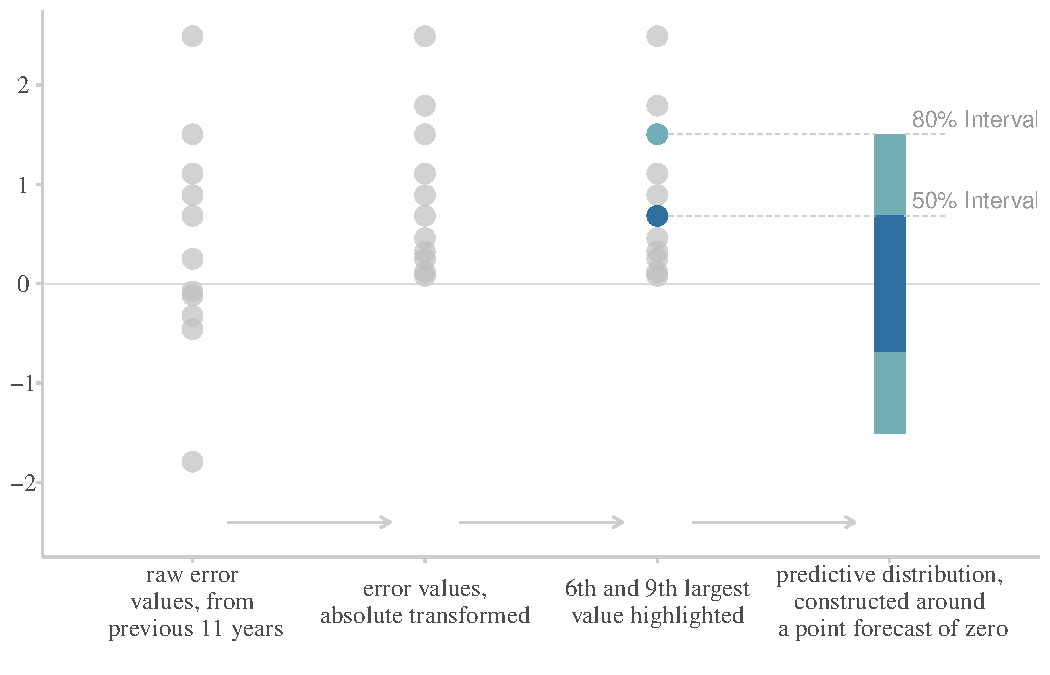
\includegraphics[width=0.65\textwidth]{figures/illustration_quantileextraction.pdf} 
        \label{fig:enter-label}
    \end{figure} 
\end{frame}

\begin{frame}{Benchmarks}
    We compare with benchmarks:
\begin{enumerate}
    \item same methodology, alternative point forecasts
    \begin{itemize}
        \item autoregressive model ("AR")
        \item Primiceri Bayesian vector autoregressive model\footnote{Primiceri, G. 2005. \textit{Time Varying Structural Vector Autoregressions and Monetary Policy.} Review of Economic Studies 72.} ("BVAR")
    \end{itemize}
    \item directly generated distributional forecasts
    \begin{itemize}
        \item obtained from the BVAR model ("BVAR - direct")
    \end{itemize}
\end{enumerate}
\begin{itemize}
    \item trained on quarterly data
\end{itemize}

\end{frame}

\section{Results}
\begin{frame}{Scores on holdout data 2013-2023 - Inflation}
%\textit{I'll make the figures, incl. legends, nicer and also remove (the reason for) the joke about the devoured overprediction}
    \begin{figure}
        \centering
        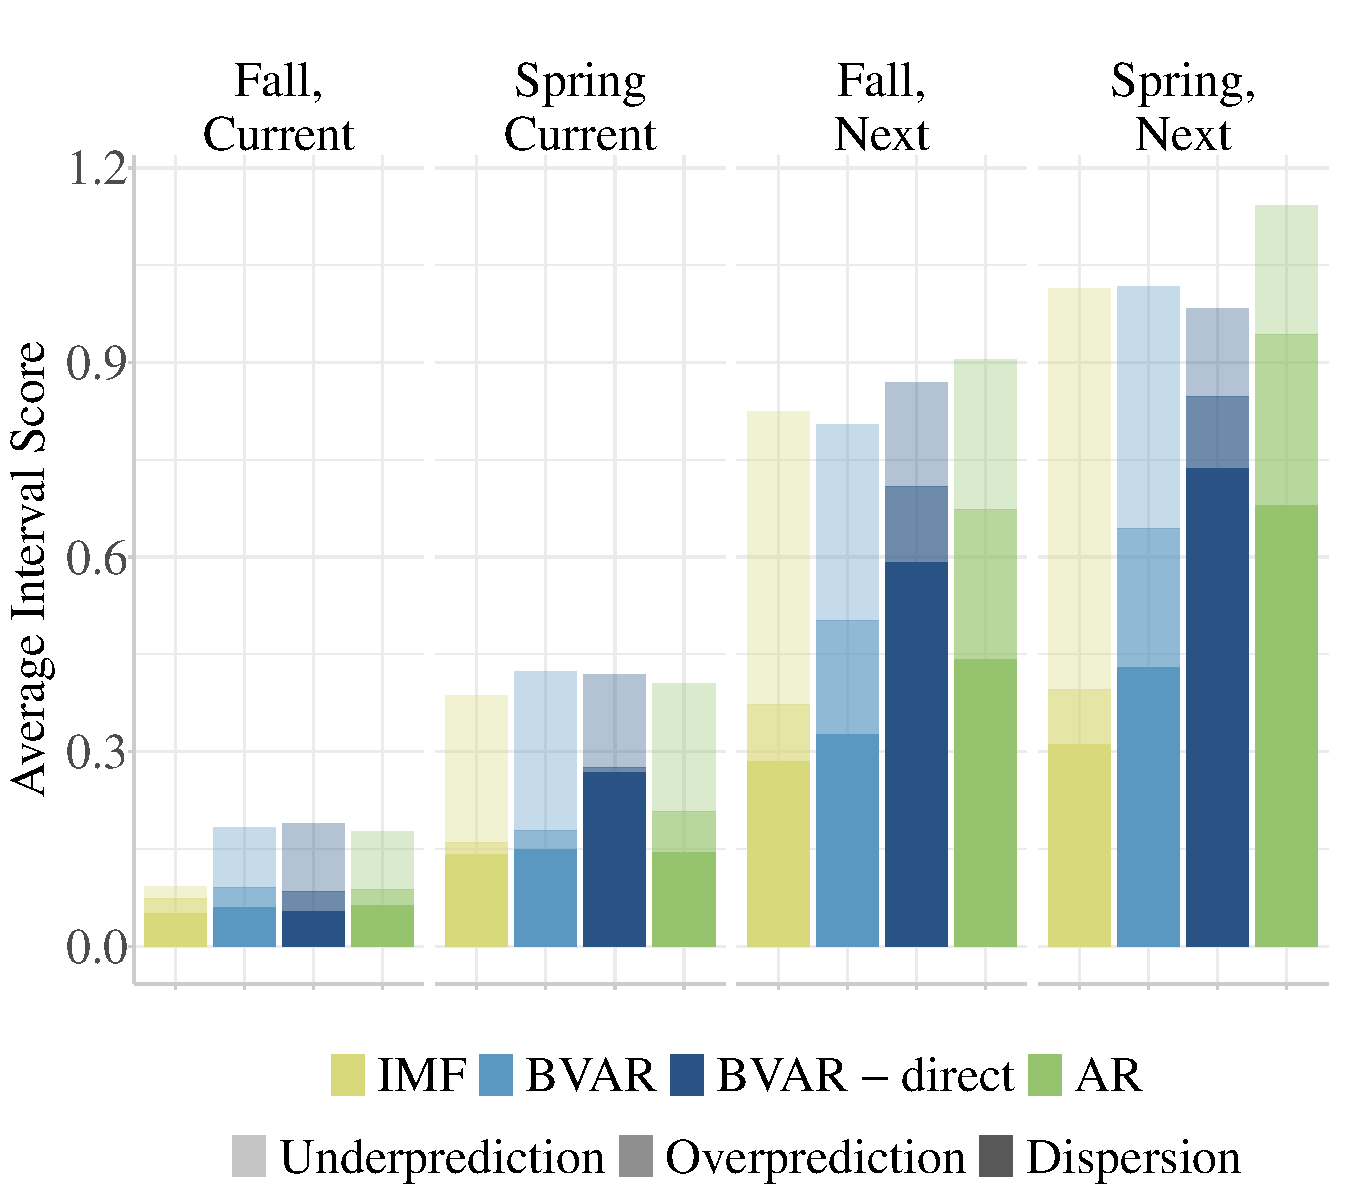
\includegraphics[width=0.45\textwidth]{figures/ho_wis_pcpi_pch_absolute_rollingwindow.pdf} 
        \label{fig:enter-label}
    \end{figure} 
\end{frame}

\begin{frame}{Scores on holdout data 2013-2023 - GDP Growth}
%\textit{I'll make the figures, incl. legends, nicer and also remove (the reason for) the joke about the devoured overprediction}
    \begin{figure}
        \centering
        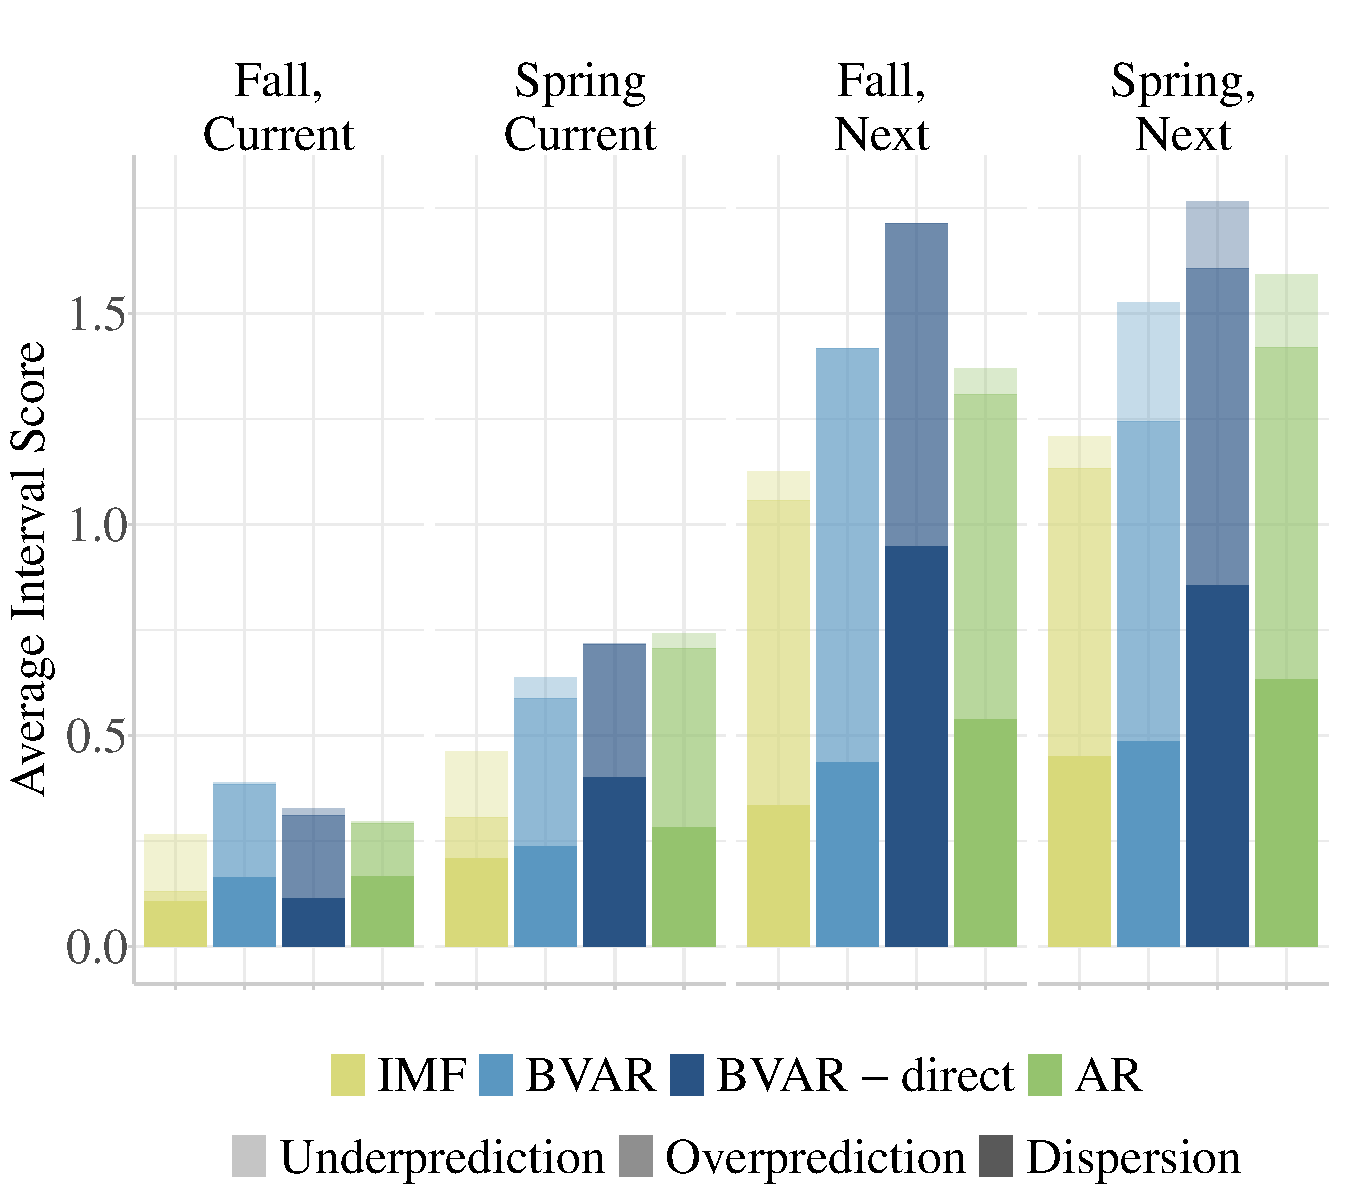
\includegraphics[width=0.45\textwidth]{figures/ho_wis_ngdp_rpch_absolute_rollingwindow.pdf} 
        \label{fig:enter-label}
    \end{figure} 
\end{frame}


\begin{frame}{Calibration - on holdout data 2013-2023}
%\textit{Here, I'll instead map the colors to the different forecast sources (currently mapped to the window method), so we'll just have one plot each}
    %Coverage at the 50\% and 80\% central interval: \\ 
\begin{figure}
  \begin{subfigure}{0.385\textwidth}
  \centering
    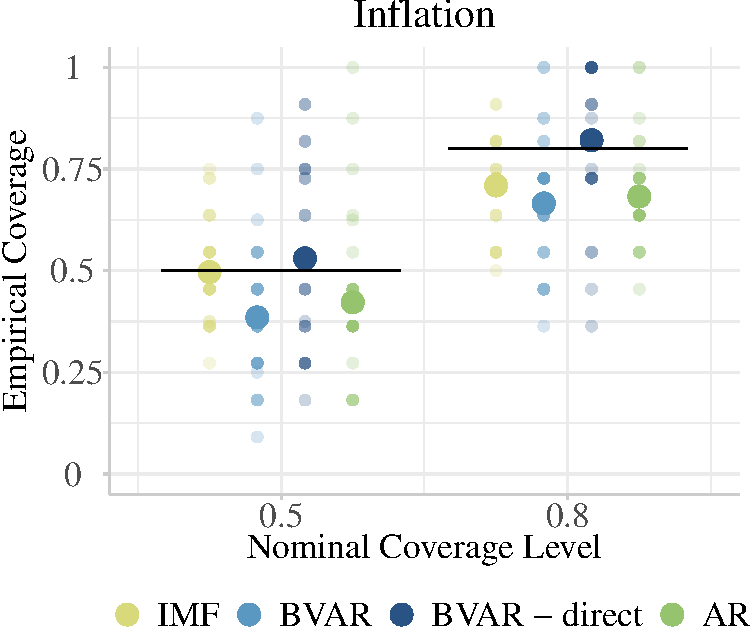
\includegraphics[width=\textwidth]{figures/ho_coverage_pcpi_pch_absolute_rollingwindow.pdf} %\vspace{0.3cm}
  \end{subfigure}
  \hspace*{12mm}
  %\hfill  % maximize separation between the subfigures
  \begin{subfigure}{0.385\textwidth}
  \centering
    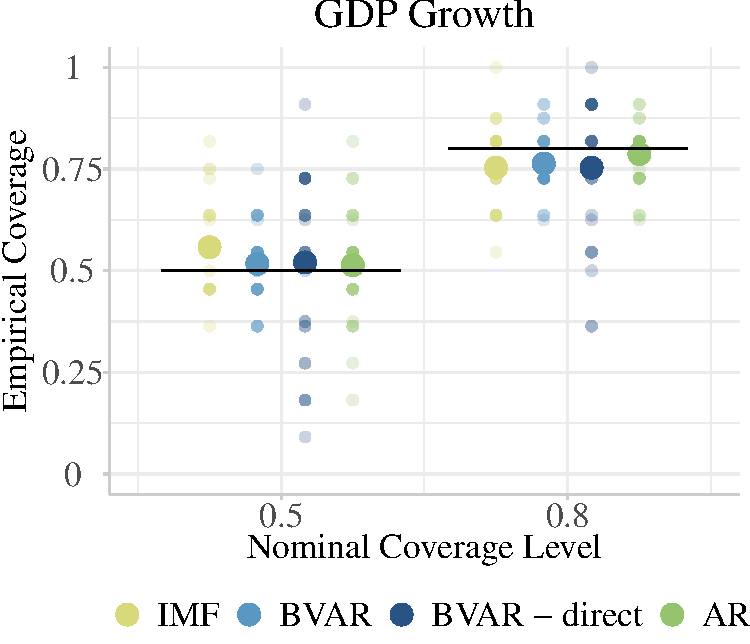
\includegraphics[width=\textwidth]{figures/ho_coverage_ngdp_rpch_absolute_rollingwindow.pdf} %\vspace{0.3cm}
  \end{subfigure}%
\end{figure}

\end{frame}

\begin{frame}{Increasing Uncertainty}
%Width of Prediction Intervals, by Horizon
%\textit{include graphic or table showing increasing uncertainty with rising horizons}\\ 
\begin{columns}
\begin{column}{0.6\textwidth}
    \begin{figure}
        \centering
        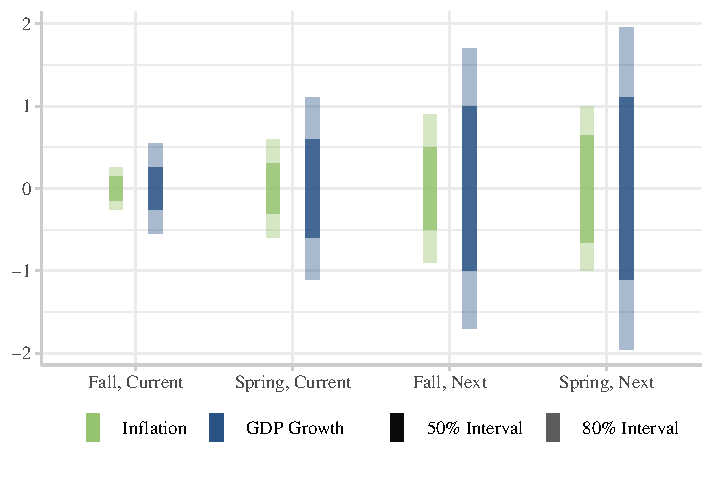
\includegraphics[width=\textwidth]{figures/cilength_byhorizon.pdf}
        %\caption{Coverage at the 50 and 80 percent level}
        \label{fig:enter-label}
    \end{figure}
\end{column}
\begin{column}{0.4\textwidth}
\centering
\textbf{Average length of intervals}
\begin{table}
\begin{tabular}{ l c c }
&   50\%  & 80\%\\[0.3em]
\multicolumn{3}{c}{\textbf{GDP Growth}}\\
Fall,  SY & 0.5 & 1.1\\ 
Spring, SY &1.0 &2.1 \\ 
Fall, NY & 1.7 & 3.3\\ 
Spring, NY &2.1 &4.0 \\[0.3em] 
\multicolumn{3}{c}{\textbf{Inflation}}\\
%&   50\%  & 80\%\\[0.3em]
Fall,  SY & 0.3 & 0.5\\ 
Spring, SY &0.6 &1.2 \\ 
Fall, NY & 1.2 & 2.0\\ 
Spring, NY &1.4 &2.2 \\ 
\end{tabular}
\end{table}
\vspace{1.25cm}
\end{column}
\end{columns}


%\textit{relate back to article shown in the beginning, which also mentions IMF forecast of 0.1 percent $\rightarrow$ almost 50\% of any predictive intervals at this time would actually be below zero}
\end{frame}
\addtocounter{framenumber}{-1}
\begin{frame}{Will Germany avoid recession?}
%Width of Prediction Intervals, by Horizon
%\textit{include graphic or table showing increasing uncertainty with rising horizons}\\ 
\begin{figure}
        \centering
        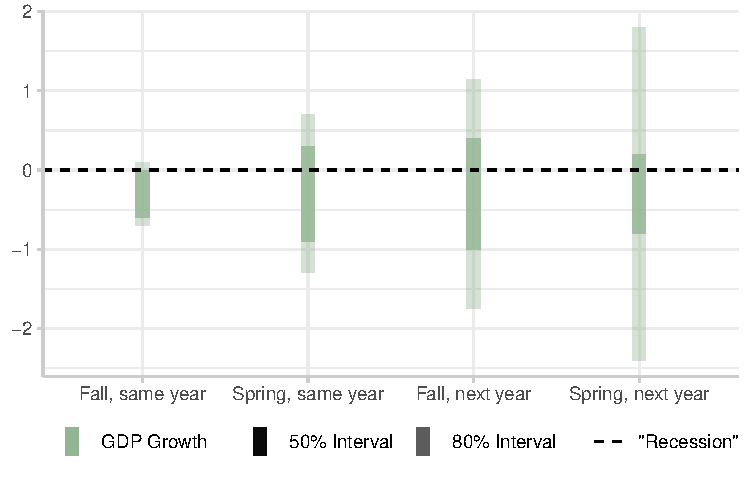
\includegraphics[width=0.6\textwidth]{figures/horizon_uncc_germany2023_current.pdf}
        %\caption{Coverage at the 50 and 80 percent level}
        \label{fig:enter-label}
    \end{figure}


%\textit{relate back to article shown in the beginning, which also mentions IMF forecast of 0.1 percent $\rightarrow$ almost 50\% of any predictive intervals at this time would actually be below zero}
\end{frame}


\begin{frame}{Robustness Checks / Alternative Methods}
\begin{itemize}
    \item error extraction method: absolute vs. directional errors
    \begin{itemize}
    \item similar scores, worse calibration \hyperlink{errorextraction}{\beamerbutton{link}}
    \end{itemize}
    \item window method: rolling vs. expanding window
    \begin{itemize}
    \item slightly improved coverage and scores, at the cost of interpretability \hyperlink{extractionmethod}{\beamerbutton{link}}
    \end{itemize}

    \item alternative truth values from the OECD
    \begin{itemize}
    \item influences evaluation results at the shortest horizon \hyperlink{alternativetruth}{\beamerbutton{link}}
    \end{itemize}
    \item alternative BVAR specification
    \begin{itemize}
    \item similar scores and calibration \hyperlink{alternativebvar}{\beamerbutton{link}}
    \end{itemize}
\end{itemize}
\end{frame}



\section{Outlook}

\begin{frame}{Summing up}
\begin{itemize}
\item Attaching distributional forecasts via past forecast errors to an existing base of point forecasts is
    \begin{itemize}
        \item cheap
        \item transparent
        \item competitive
    \end{itemize}
\item IMF forecasts are valuable source for distributional forecasts 
\item Uncertainty around point forecasts is often substantial, making its communication necessary\bigskip \\
\item Potential Extensions / Outlook
    \begin{itemize}
        \item scale to more countries
        %\item implement alternative method that  utilizes the cross-section dimension%, e.g. via Hierarchical Bayesian Modeling
        \item make forecasts easily and publicly accessible via shiny app
        \item preregistration of real-time forecasts
    \end{itemize}

\end{itemize}
\end{frame}

\begin{frame}{Making it public}
\begin{columns}
\begin{column}{0.3\textwidth}
Shiny App: \\
   \url{https://probability-forecasting.shinyapps.io/macropi/} \vspace{0.5cm} \\ 
GitHub repo with our forecasts: \\
    \url{https://github.com/MacroPrediction/MacroPI}
    \vspace*{2cm}
\end{column}
\begin{column}{0.7\textwidth}
\vspace*{-10mm}
    \begin{figure}
        %\centering
        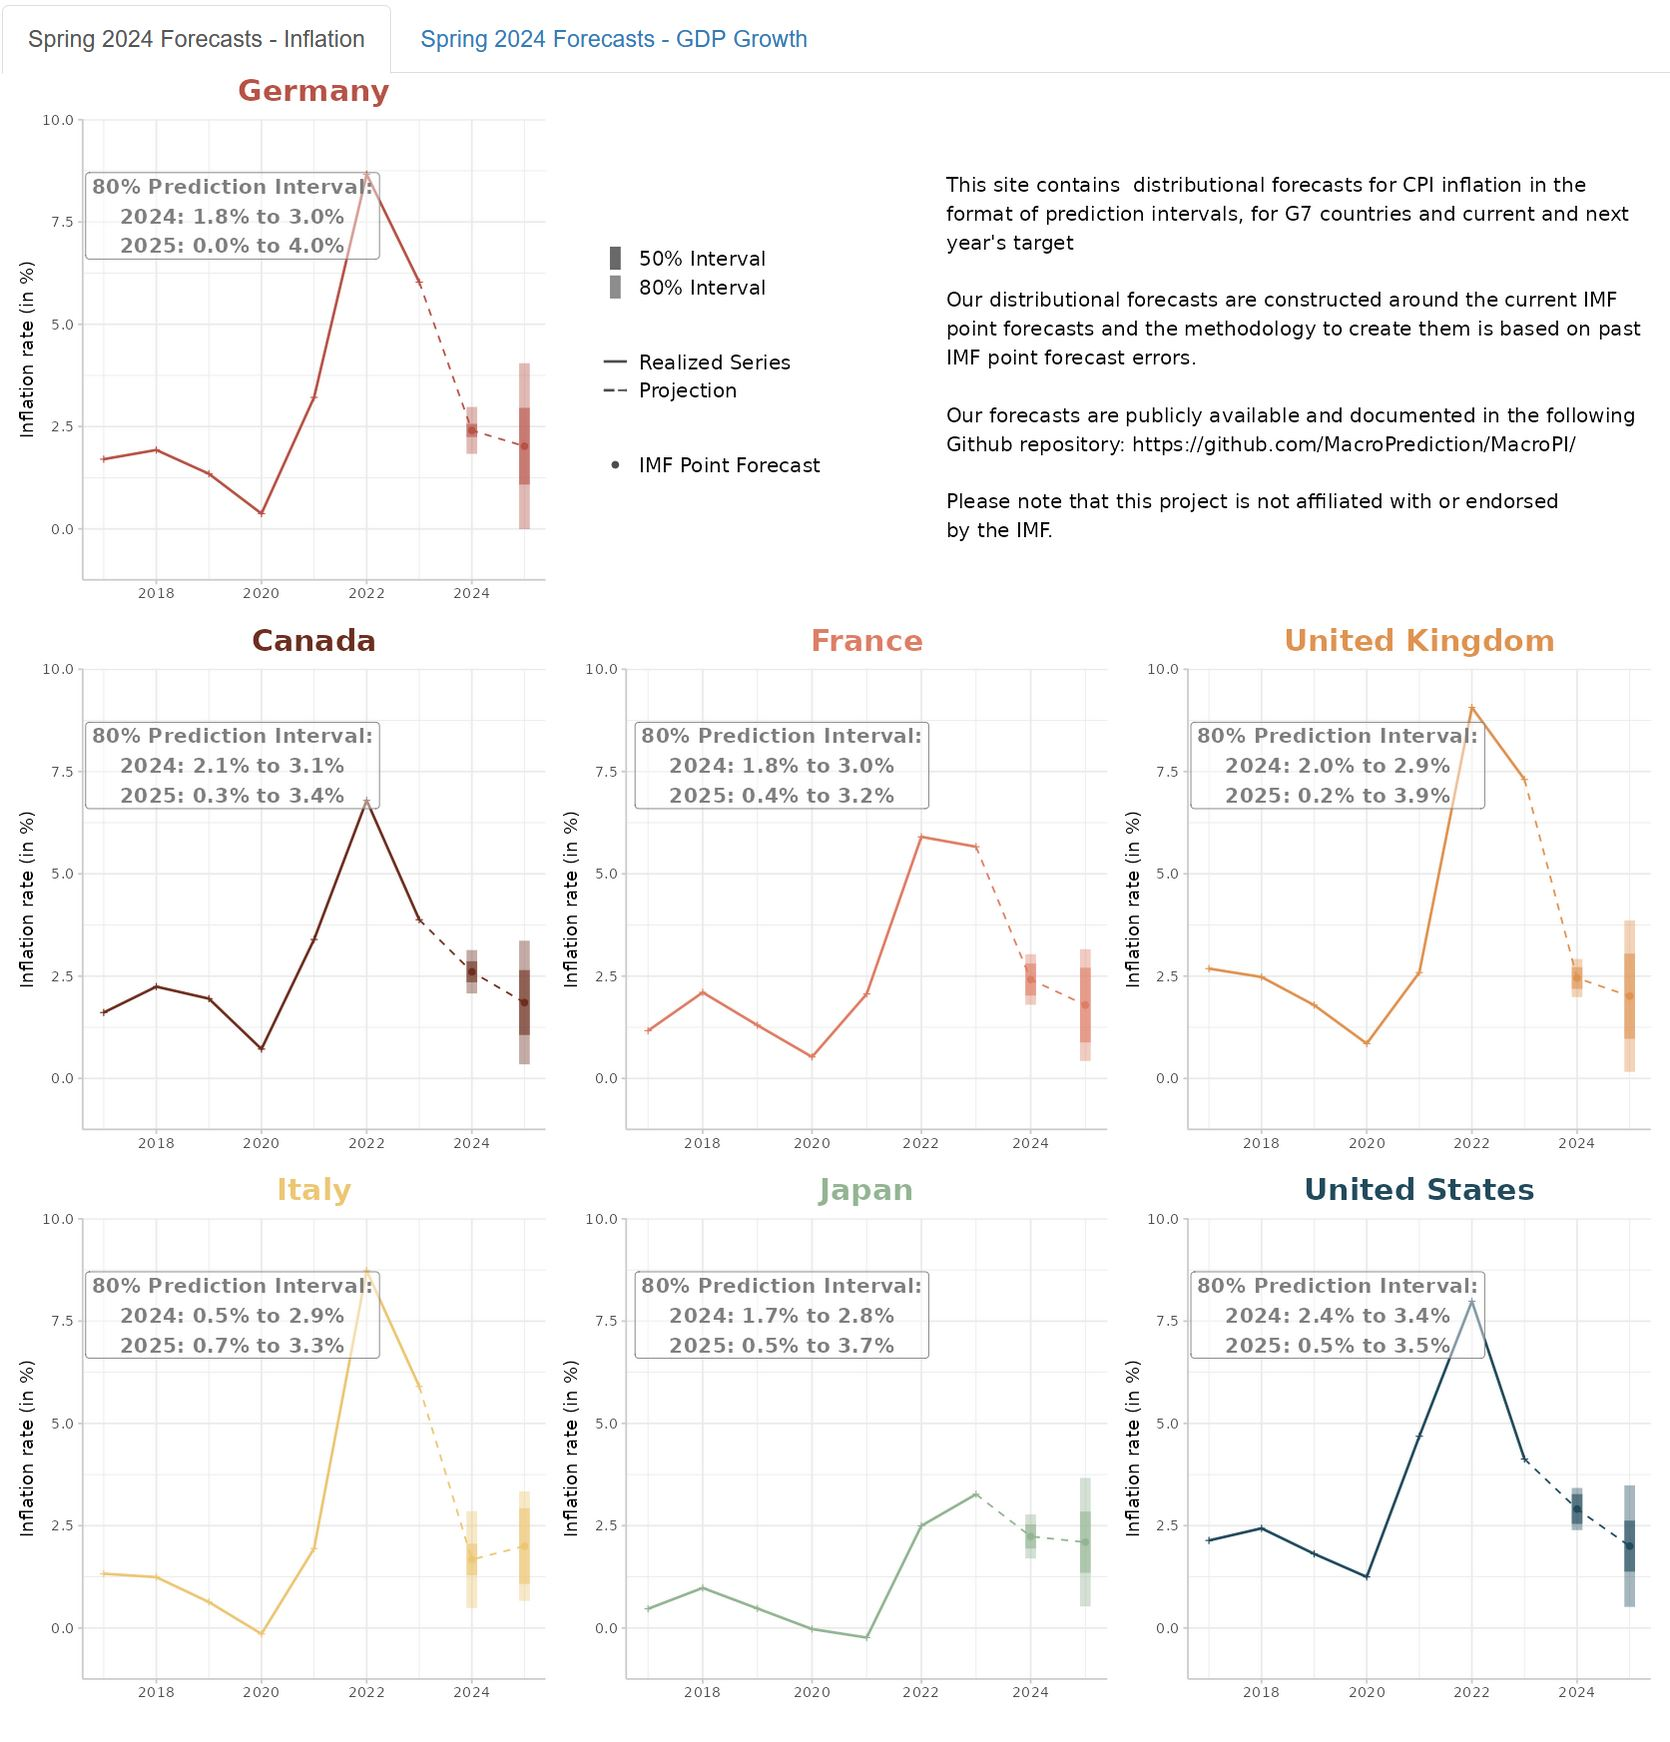
\includegraphics[width=0.55\textwidth]{figures/shinycap_final.jpg}
        %\caption{Coverage at the 50 and 80 percent level}
        \label{fig:enter-label}
    \end{figure}   
\end{column}
\end{columns}

\end{frame}

\begin{frame}{Making it public - Timestamped Forecast Publication I}

    \begin{figure}
        %\centering
        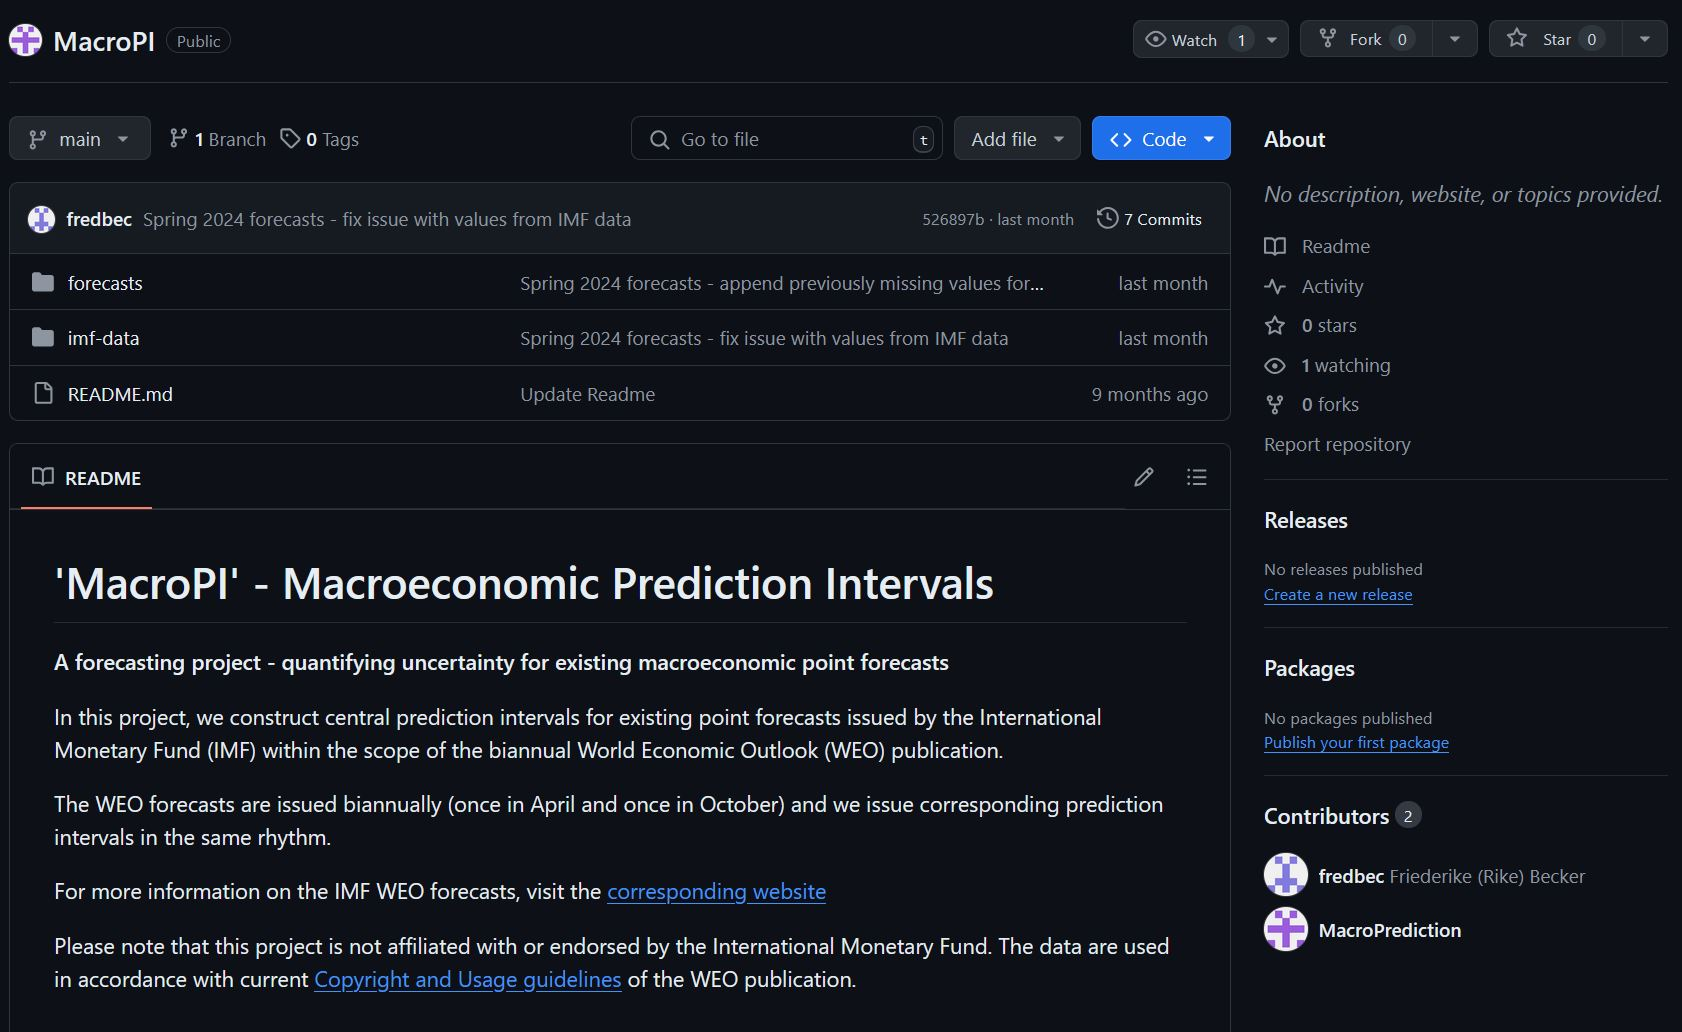
\includegraphics[width=0.65\textwidth]{figures/Capture_GitHub.jpg}
        %\caption{Coverage at the 50 and 80 percent level}
        \label{fig:enter-label}
    \end{figure}   

\end{frame}

\begin{frame}{Making it public - Timestamped Forecast Publication II}

    \begin{figure}
        %\centering
        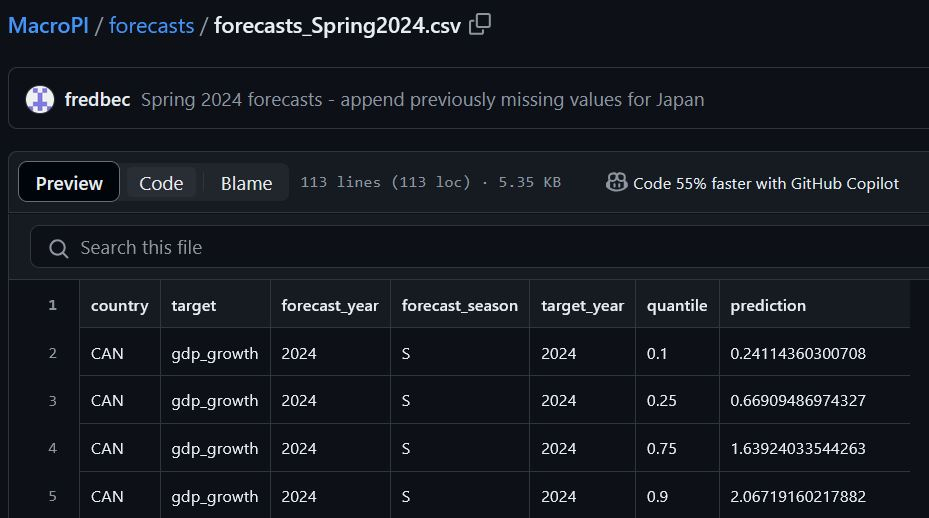
\includegraphics[width=0.65\textwidth]{figures/Capture_GitHubforecasts.jpg}
        %\caption{Coverage at the 50 and 80 percent level}
        \label{fig:enter-label}
    \end{figure}   

\end{frame}

\begin{frame}{Making it public - Visualization}

    \begin{figure}
        %\centering
        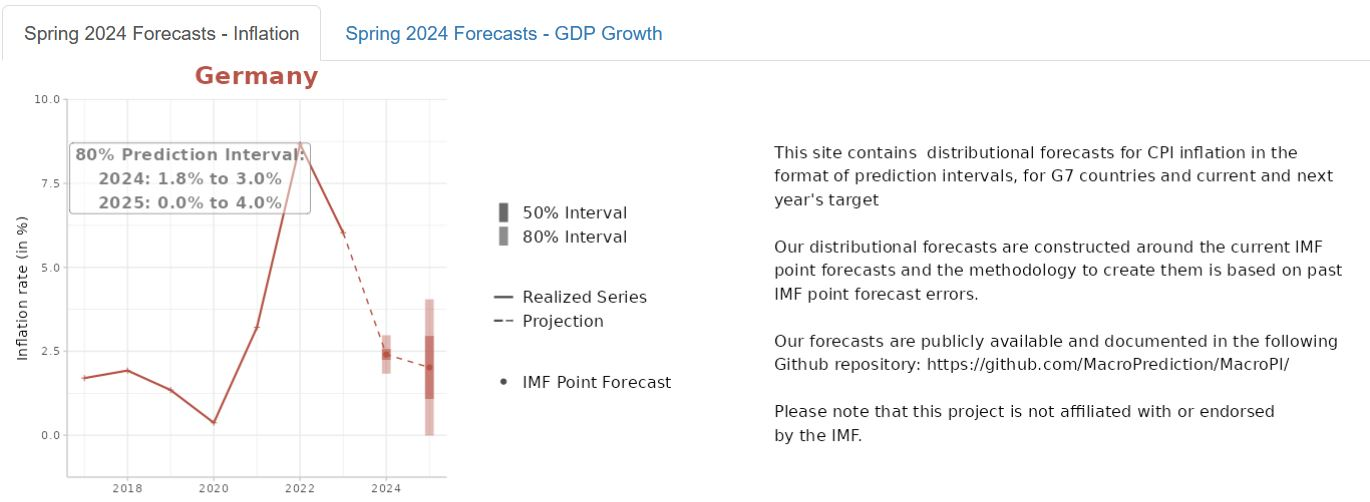
\includegraphics[width=0.85\textwidth]{figures/shinycap_enlarged.jpg}
        %\caption{Coverage at the 50 and 80 percent level}
        \label{fig:enter-label}
    \end{figure}   

\end{frame}

%\begin{frame}{Beispielinhalt: Literatur}
%    Literaturzitat: \cite{klare2021jss}
%end{frame}
%\begin{frame}
%        Bei Frames ohne Titel wird die Kopfzeile nicht angezeigt, und  
%    der freie Platz kann für Inhalte genutzt werden.
%\end{frame}

%\begin{frame}[plain]
%    Bei Frames mit Option \texttt{[plain]} werden weder Kopf- noch Fußzeile angezeigt.
%\end{frame}

%\begin{frame}[t]{Beispielinhalt}
%    Bei Frames mit Option \texttt{[t]} werden die Inhalte nicht vertikal zentriert, sondern an der Oberkante begonnen.
%\end{frame}

\appendix
\beginbackup
\begin{frame}{Directional Errors - Scores on years 2001-2012}
\label{errorextraction}
\begin{table}
\begin{center}
\begin{tabular}{lccccccc}
 & & \multicolumn{2}{c}{Interval Score} & \multicolumn{2}{c}{50\% Cvg.} & \multicolumn{2}{c}{80\% Cvg.} \\[0.2em]
 & Horizon & absolute & directional & absolute & directional & absolute & directional\\[0.5em]
\multirow{4}{*}{\rotatebox[origin=c]{90}{GDP Growth}} & Fall, Current & \textbf{0.23} & 0.24 & \textbf{0.49} & 0.43 & \textbf{0.76} & 0.65\\
 & Spring, Current & 0.41 & \textbf{0.41} & 0.56 & \textbf{0.54} & \textbf{0.76} & 0.67\\
 & Fall, Next & 0.91 & \textbf{0.88} & \textbf{0.49} & 0.42 & \textbf{0.73} & 0.70\\
 & Spring, Next & \textbf{1.14} & 1.15 & \textbf{0.50} & 0.40 & \textbf{0.64} & 0.55\\[1em]
\multirow{4}{*}{\rotatebox[origin=c]{90}{Inflation}} & Fall, Current & \textbf{0.12} & 0.12 & \textbf{0.52} & 0.44 & \textbf{0.76} & 0.64\\
 & Spring, Current & 0.26 & \textbf{0.25} & \textbf{0.43} & 0.39 & \textbf{0.75} & 0.65\\
& Fall, Next & \textbf{0.47} & 0.50 & \textbf{0.40} & 0.31 & \textbf{0.67} & 0.54\\
 & Spring, Next & \textbf{0.52} & 0.55 & \textbf{0.42} & 0.38 & \textbf{0.67} & 0.54\\


\end{tabular}
\end{center}
\end{table}
\end{frame}



\begin{frame}{Expanding Window - Scores}
\label{extractionmethod}
\end{frame}

\begin{frame}{Alternative truth value - Scores}
\label{alternativetruth}
    \begin{figure}
        %\centering
        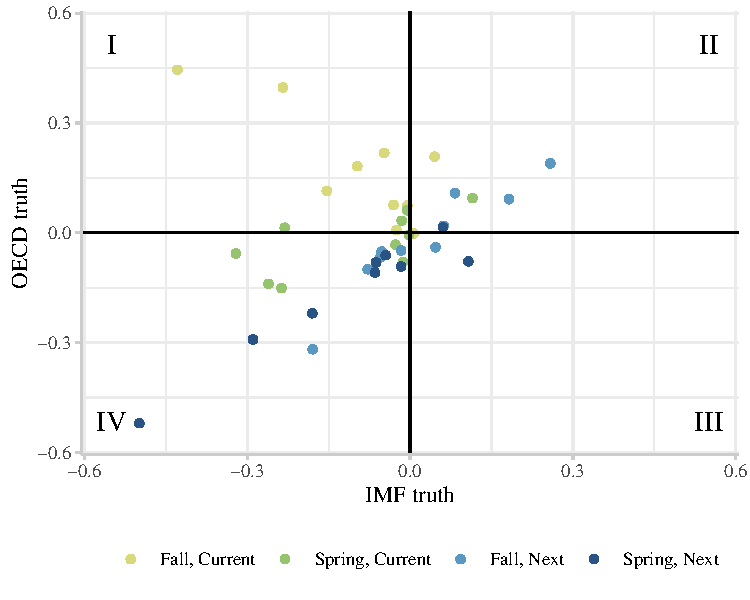
\includegraphics[width=0.55\textwidth]{figures/oecdvsimf.pdf}
        %\caption{Coverage at the 50 and 80 percent level}
        \label{fig:enter-label}
    \end{figure}   
\end{frame}

\begin{frame}{Alternative BVAR specification - Scores}
\label{alternativebvar}
\begin{figure}
  \begin{subfigure}{0.45\textwidth}
  \centering
    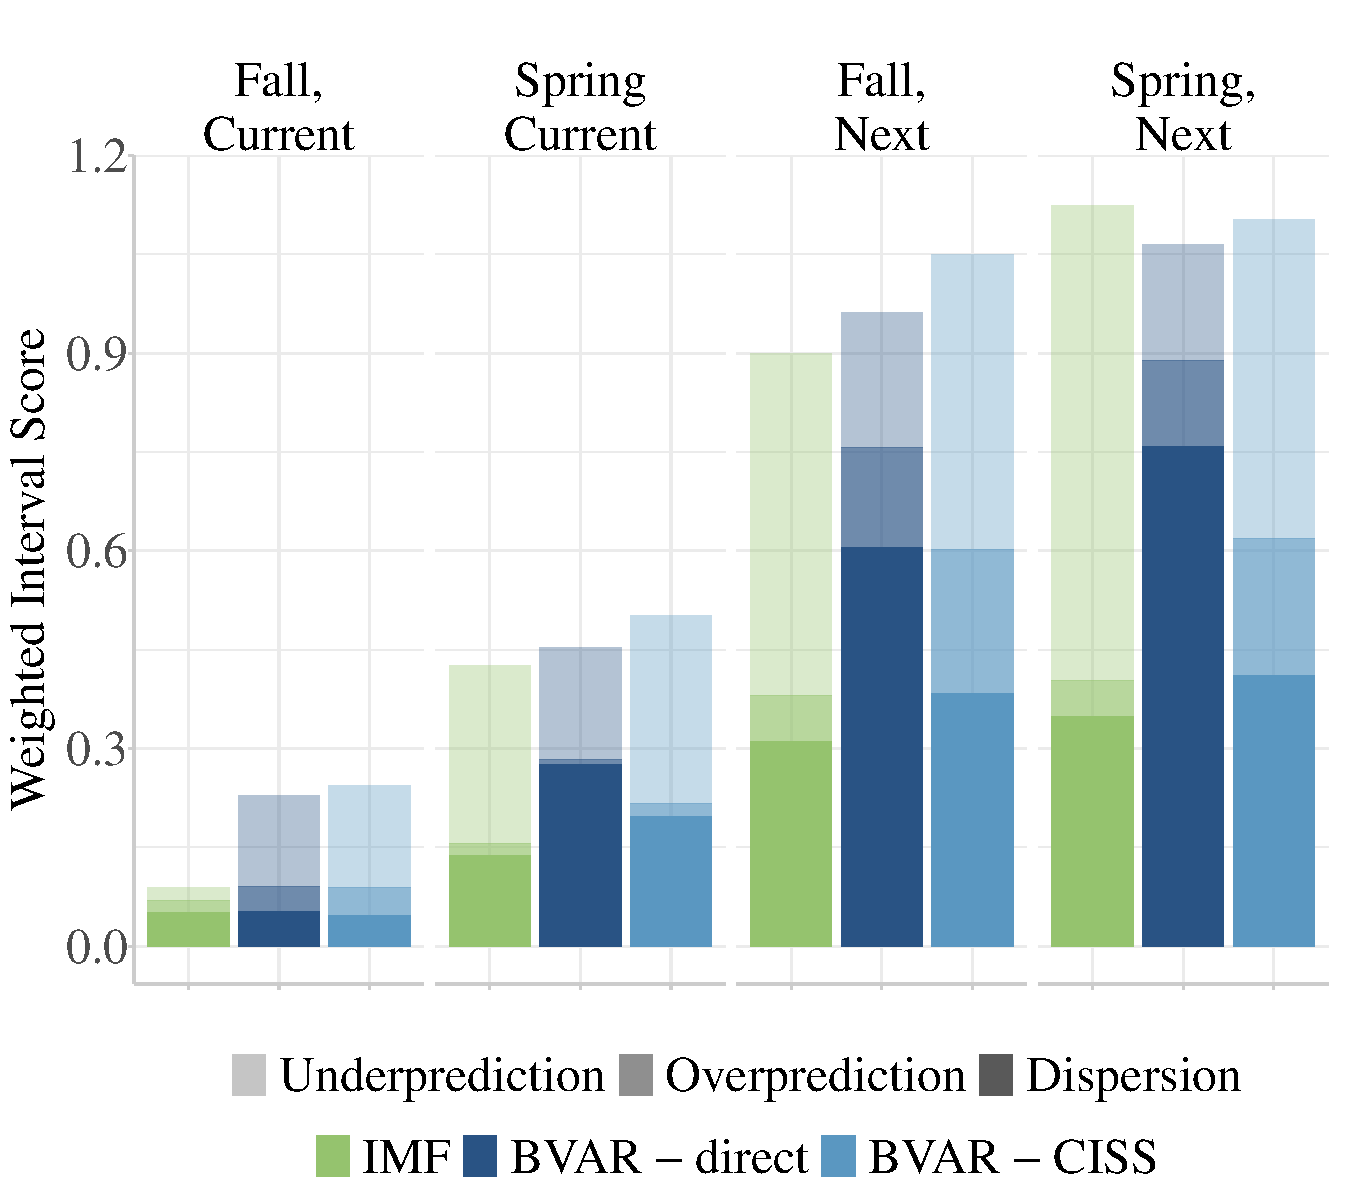
\includegraphics[width=\textwidth]{figures/ho_bvarspecs_wis_pcpi_pch_absolute_rollingwindow.pdf} %\vspace{0.3cm}
    \caption{Inflation}
  \end{subfigure}
  \hspace*{8mm}
  %\hfill  % maximize separation between the subfigures
  \begin{subfigure}{0.45\textwidth}
  \centering
    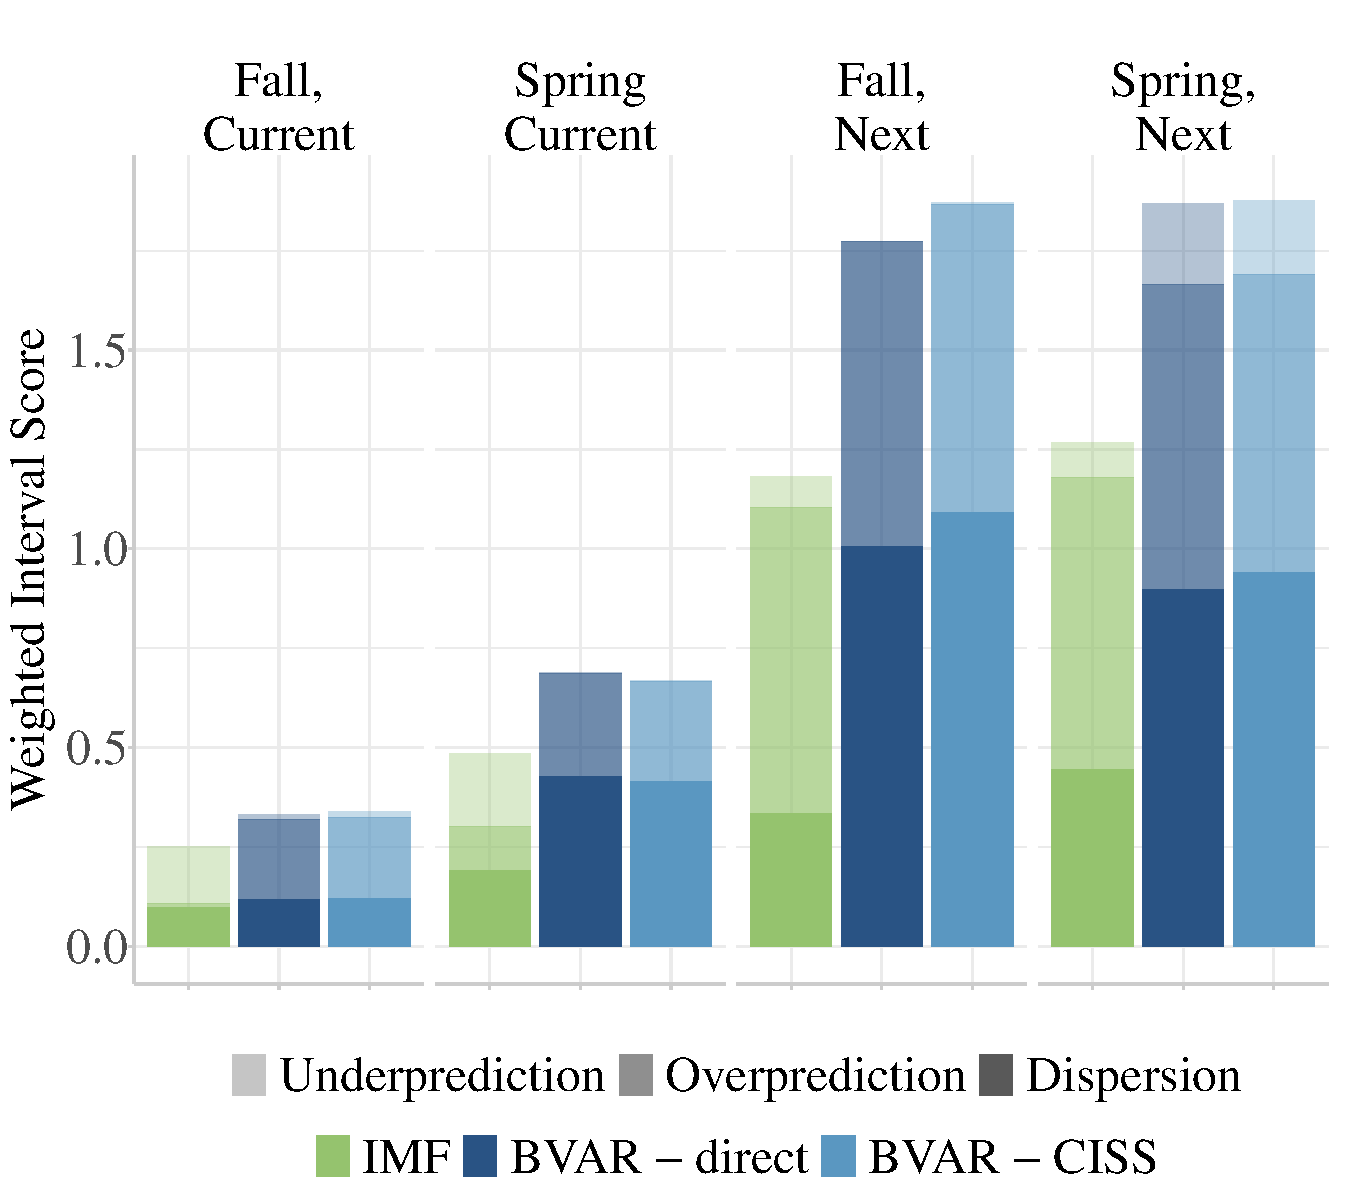
\includegraphics[width=\textwidth]{figures/ho_bvarspecs_wis_ngdp_rpch_absolute_rollingwindow.pdf} %\vspace{0.3cm}
    \caption{GDP Growth}
  \end{subfigure}%
\end{figure}
\end{frame}



%\begin{frame}{Literatur}
%\begin{exampleblock}{Backup-Teil}
%    Folien, die nach \texttt{\textbackslash beginbackup} eingefügt werden, zählen nicht in die Gesamtzahl der Folien.
%\end{exampleblock}

%\printbibliography
%\end{frame}

%\section{Farben}
%% ----------------------------------------
%% | Test-Folie mit definierten Farben |
%% ----------------------------------------
%% ----------------------------------------
%% | /Test-Folie mit definierten Farben |
%% ----------------------------------------
\backupend

\end{document}